\documentclass[addpoints,12pt]{exam}
%\documentclass[12pt]{article}
\usepackage[letterpaper, margin=0.75in]{geometry}
\usepackage{graphicx}
\usepackage{enumitem}
\usepackage{booktabs}
\usepackage{tabularx}
\usepackage{color}
\usepackage{wrapfig}

\begin{document}
\footer{}{Page \thepage\ of \numpages}{}



\begin{center}

\includegraphics[width=10cm]{../images/logo.png}
\end{center}

\begin{center}
\noindent{\LARGE Conceptual Physics \\ Second Partial Test\\ \textbf{SOLUTIONS} \\ May 18, 2018 \\}
\end{center}

\vspace{0.5in}




 
\clearpage

\begin{flushright}
Score: \hspace{0.2in} / \numpoints ~ points
\end{flushright}

\begin{questions}
\question \textbf{Drawing Field Lines:} Six particles are arranged on a hexagon. They all have identical masses. Some are positively charged, and some are negatively charged. They all have charge of $\pm 1$ (so the size of all charges are the same).

\begin{parts}

\part[2] Draw the \textbf{electric field} lines around the particles. If there is a point with \textbf{zero} electric field, indicated it on the diagram.
\vspace{1in}
\begin{center}
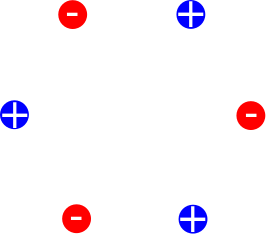
\includegraphics[width=2in]{../images/hexagonCharges.png}
\end{center}
\vspace{1in}

\part[2] Draw the \textbf{gravitational field} lines around the particles. If there is a point with \textbf{zero} gravitational field, indicated it on the diagram.
\vspace{1in}
\begin{center}
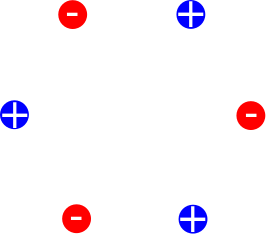
\includegraphics[width=2in]{../images/hexagonCharges.png}
\end{center}
\vspace{1in}
\end{parts}

\clearpage
\question \textbf{Alien Planet:} On a distant planet, aliens have set up a monitoring post with two lasers that are distance \textit{D} apart. They see a spaceship traveling at 1/3 the speed of light, passing over their lasers and decide to fire at the ship, creating scorch marks on the ship's hull. T\textbf{he image below shows this setup from the perspective of an alien on the planet.}

\begin{center}
\input{../images/firingSpaceship.pdf_tex}
\end{center}
	\begin{parts}
		\part[2] The aliens on the planet fire the lasers at the same time. How far apart would they say the scorch marks on the ship are?
			\begin{choices}
				\choice Exactly a distance \textit{D} apart.
				\choice A distance greater than \textit{D} apart.
				\choice A distance less than \textit{D} apart.
			\end{choices}
			\begin{TheSolution}
				\textbf{A.} Since the lasers were fired at the same time, the laser beams would both point directly up and always be a distance \textit{D} apart: therefore when the hit the ship, they will be a distance \textit{D} apart.
			\end{TheSolution}
		\part[2] From the perspective of an alien \textit{on the ship}, how far apart are the scorch marks on the ship?
			\begin{choices}
				\choice Exactly a distance \textit{D} apart.
				\choice A distance greater than \textit{D} apart.
				\choice A distance less than \textit{D} apart.
			\end{choices}
			\begin{TheSolution}
				\textbf{B.} To an alien on the planet, the ship is length contracted (which is why it appears squished in the diagram). All ship-measurements to an alien on the ship will therefore be longer than the measurements made by an alien on the planet, including the distance between scorch marks.
			\end{TheSolution}
		\part[2] From the perspective of an alien \textit{on the ship}, how far apart are the laser cannons on the planet?
			\begin{choices}
				\choice Exactly a distance \textit{D} apart.
				\choice A distance greater than \textit{D} apart.
				\choice A distance less than \textit{D} apart.
			\end{choices}
			\begin{TheSolution}
			\textbf{C.} To an alien on the ship, they are stationary and the planet is moving: therefore length on the planet will be contracted from their perspective. As a result, they will see the laser cannons closer together than would an alien on the planet.
			\end{TheSolution}
		\part[2] An alien on the planet says that the laser beams strike the ship simultaneously. Would an alien on the ship agree?
			\begin{choices}
				\choice Yes, the lasers were fired at the same time and so they would agree.
				\choice No, they would say the beam from laser A struck first.
				\choice No, they would say the beam from laser B struck first.
			\end{choices}
			\begin{TheSolution}
			\textbf{B.} To an alien on the ship, the distance between the scorch marks is greater than \textit{D} but the distance between the cannons is less than \textit{D.} The only way for this to be possible is if the two lasers did not fire simultaneously. Laser \textit{A} would have had to fire first.
			\end{TheSolution}
	\end{parts}


\question \textbf{Quark Energies:} Quarks are elementary particles (meaning that, to our knowledge, they cannot be broken down). Three quarks can come together to make up a proton or a neutron, and because there are different kinds of quarks the different combinations can yield different particles. There are 6 different quarks, each with a different mass:

\begin{tabular}{l l }
	up quark & $4.30 \times 10^{-30}$ kg \\
	down quark & $8.59 \times 10^{-30}$ kg \\
	charm quark & $2.28 \times 10^{-27}$ kg\\
	strange quark & $1.70 \times 10^{-28}$ kg \\
	top quark & $3.09 \times 10^{-25}$ kg \\
	bottom quark & $7.48 \times 10^{-27}$ kg
\end{tabular}

\begin{parts}
	\part[2] Considering Einstein's equation which relates mass to energy, $E=mc^2$, which quark has the \textbf{most} mass-energy?
		\begin{TheSolution}
		\textbf{Top Quark.} The quark with the most mass will have the most energy. The top quark is about 100 to 100,000 times more massive than any other quark, and so is by far the most massive.
		\end{TheSolution}
	\part[2] Considering Einstein's equation which relates mass to energy, $E=mc^2$, which quark has the \textbf{least} mass-energy?
		\begin{TheSolution}
		\textbf{Up Quark.} The up and down quarks have masses on the order of $10^{-30}$, which is about 1000 to 100,000 times less massive than the other 4. Of the two, the up quark is slightly smaller at $4.30 \times 10^{-30}$ kg compared to $8.59 \times 10^{-30}$ kg for the down quark.
		\end{TheSolution}
	\part[2] By the principle of wave-particle duality, we know that these different quarks also have different wavelengths. Below are six different waves (shown with decreasing wavelength), which represent the wavelengths of these different quarks (assuming their velocities are negligible). Label them.
	\begin{center}
	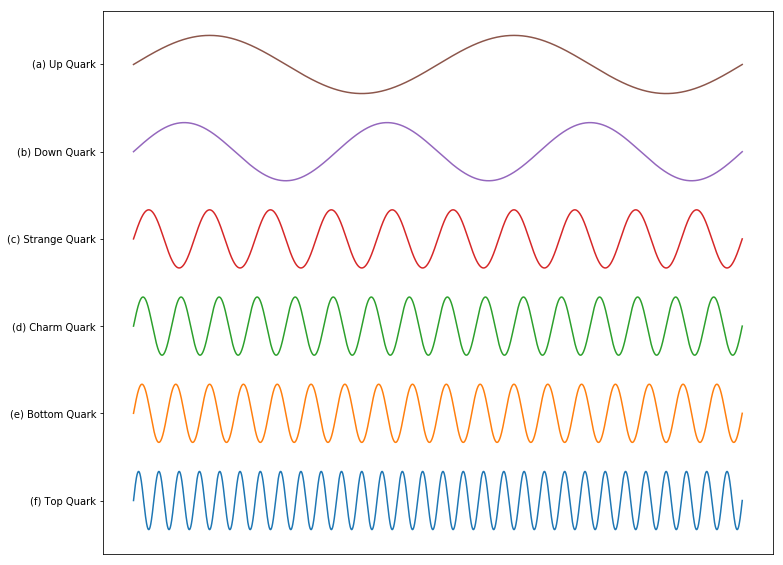
\includegraphics[width=0.9\textwidth]{../images/quarksWavesSol.png}
	\end{center}
\end{parts}

	\begin{center}
	\noindent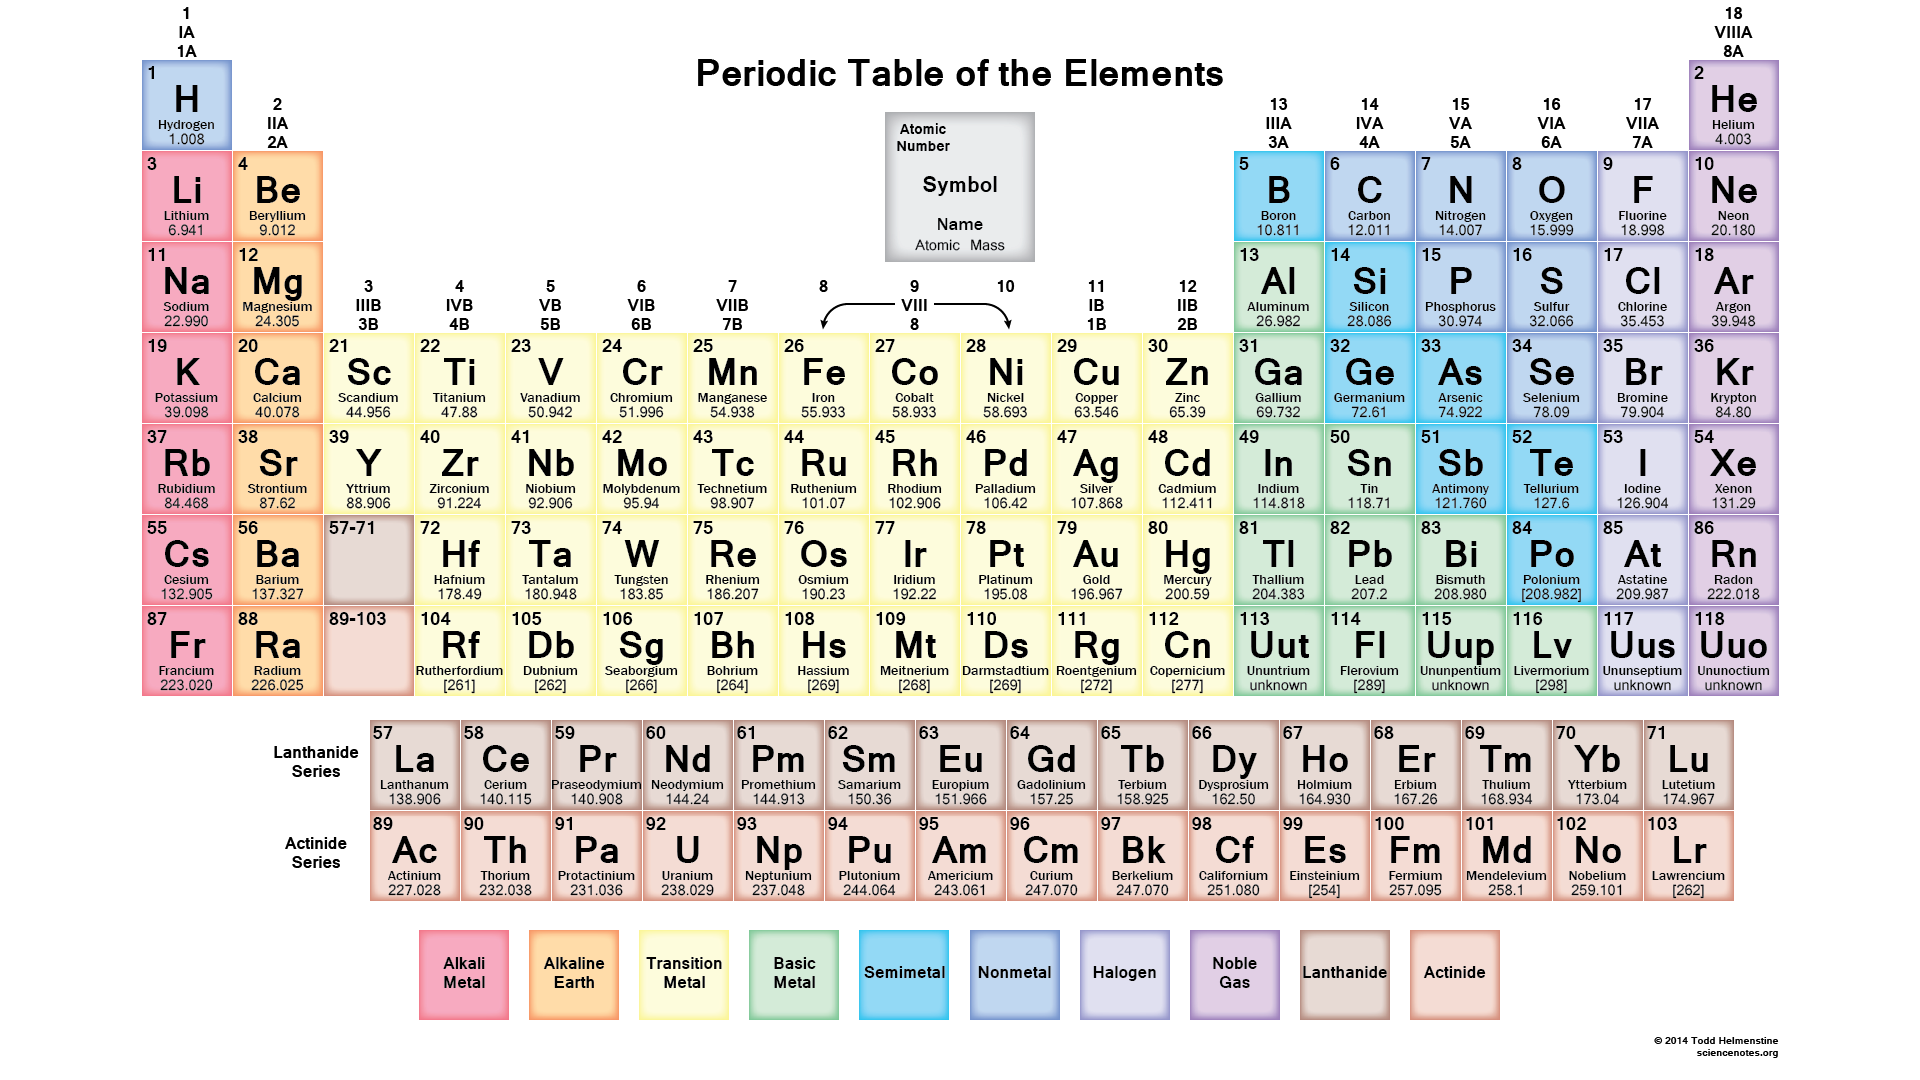
\includegraphics[width=\textwidth]{../images/periodicTable.png}
	\end{center}
	
	\question \textbf{Uranium Decays:} Uranium-238 decays via alpha decay (where it emits a Helium-4 nucleus).
	\begin{center}
		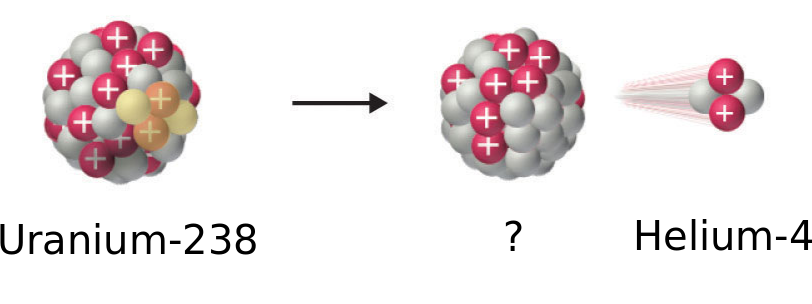
\includegraphics[width=2.5in]{../images/uraniumAlpha.png}
	\end{center}

	
\begin{parts}
\part[2] What element does uranium-238 decay to?
\begin{TheSolution}
	\textbf{Thorium.} Specifically, Thorium-234 ($^{234}Th$). By losing a helium-4 nucleus, the uranium-238 nucleus lost 2 protons, and so goes down 2 on the periodic table. This is Thorium. Since it lost 4 nucleons (2 protons and 2 neutrons) the mass number goes down by 4.
\end{TheSolution}
\part[2] How many protons and neutrons does this decay product have?
\begin{TheSolution}
	\textbf{90 Protons and 144 Neutrons.} Uranium-238 has 92 protons and (238 - 92 = 146) neutron. When it decays, it loses 2 protons and 2 neutrons, so the remaining thorium nucleus will have 90 protons and 144 neutrons.
\end{TheSolution}
\part[2] The half-life of uranium-238 is about 5 billion years. After 15 billion years, what fraction of a block of uranium-238 will \textbf{remain}?
\begin{TheSolution}
	\textbf{1/8 or 0.125} Since 15 billion years is 3 half lives, ($3\times 5 = 15$) the amount of uranium-238 that will remain will be
	\begin{eqnarray*}
		\frac{1}{2}\times \frac{1}{2} \times \frac{1}{2} = \frac{1}{8} = 0.125
	\end{eqnarray*}
\end{TheSolution}
\part[2] The half-life of uranium-238 is about 5 billion years. After 20 billion years, what fraction of a block of uranium-238 will have \textbf{decayed}?
\begin{TheSolution}
	\textbf{15/16 or 0.9375} Since 20 billion years is 4 half-lives, the amount of uranium that will remain will be
	\begin{eqnarray*}
		\frac{1}{2} \times \frac{1}{2} \times \frac{1}{2} \times \frac{1}{2} = \frac{1}{16}
	\end{eqnarray*}
	This means that the fraction that will have decayed is:
	\begin{eqnarray*}
		1 - \frac{1}{16} = \frac{15}{16} = 0.9375
	\end{eqnarray*}
\end{TheSolution}
\end{parts}

\question \textbf{Black Holes:} Suppose scientists on Earth decide to launch two satellites at a black hole. Both satellites are identical, and transmit information via radio waves, which observers on Earth can detect. Both satellites are in an identical orbit around the black hole (so \textit{they are stationary with respect to each other}), just outside the event horizon.

\begin{center}
\input{../images/blackHoleTwoProbe.pdf_tex}
\end{center}
\begin{parts}
\part[1] Satellite \textit{A} emits two radio pulses, 5 seconds apart. To an observer on Earth, who is watching the satellite and detecting the pulses,
\begin{choices}
	\choice The timing between pulses is also 5 seconds.
	\choice The timing between pulses is greater than 5 seconds.
	\choice The timing between pulses is less than 5 seconds.
\end{choices}
\begin{TheSolution}
	\textbf{B.} Since the satellite is in a much stronger gravitational field than Earth, because it is so close to a black hole, there is a huge time dilation. This means time is ``stretched out" more: or things will take a lot longer, and so the time between pulses will be much greater than 5 seconds.
\end{TheSolution}
\part[1] Satellite \textit{A} emits two radio pulses, 5 seconds apart. To an observer on satellite \textit{B}, who is able to observe satellite \textit{A},
\begin{choices}
	\choice The timing between pulses is also 5 seconds.
	\choice The timing between pulses is greater than 5 seconds.
	\choice The timing between pulses is less than 5 seconds.
\end{choices}
\begin{TheSolution}
	\textbf{A.} Since the two satellites are the same distance away from the black hole they are in the same gravitational field, and thus there is no time dilation between the two, and so they will observe the passage of time to be the same.
\end{TheSolution}
\part[1] The frequency of radio waves emitted by satellite \textit{A} is 5 MHz. To an observer on Earth, who is watching the satellite and detecting the light,
\begin{choices}
	\choice The frequency of the radio waves is also 5 MHz.
	\choice The frequency of the radio waves is greater than 5 MHz.
	\choice The frequency of the radio waves is less than 5 MHz.
\end{choices}
\begin{TheSolution}
	\textbf{C.} Since radio waves are light, as they rise up and out of the gravitational well created by the black hole they are red-shifted: meaning they have a much longer wavelength and shorter frequency when they arrive at Earth.
\end{TheSolution}
\part[1] The frequency of radio waves emitted by satellite \textit{A} is 5 MHz. To an observer on satellite \textit{B}, who is able to detect the light from satellite \textit{A},
\begin{choices}
	\choice The frequency of the radio waves is also 5 MHz seconds.
	\choice The frequency of the radio waves is greater than 5 MHz seconds.
	\choice The frequency of the radio waves is less than 5 MHz seconds.
\end{choices}
\begin{TheSolution}
	\textbf{A.} Since the satellites are in the same gravitational field, there is no red/blue shift resulting from a change in gravitational field. Since they are not moving with respect to each other, there is also no red/blue shift coming from a Doppler effect, and so they will both measure the light to have the same frequency and wavelength.
\end{TheSolution}
\clearpage
\part[1] The frequency of radio waves emitted by satellite \textit{A} is 5 MHz. To an observer on Earth, who is watching the satellite and detecting the light,
\begin{choices}
	\choice The radio waves coming from satellite \textit{A} are traveling at the speed of light.
	\choice The radio waves coming from satellite \textit{A} are traveling slower than the speed of light.
	\choice The radio waves coming from satellite \textit{A} are traveling faster than the speed of light.
\end{choices}
\begin{TheSolution}
	\textbf{A.} Light is always traveling at the speed of light, to any observer.
\end{TheSolution}
\part[1] The frequency of radio emitted waves by satellite \textit{A} is 5 MHz. To an observer on satellite \textit{B}, who is watching the satellite and detecting the light,
\begin{choices}
	\choice The radio waves coming from satellite \textit{A} are traveling at the speed of light.
	\choice The radio waves coming from satellite \textit{A} are traveling slower than the speed of light.
	\choice The radio waves coming from satellite \textit{A} are traveling faster than the speed of light.
\end{choices}
\begin{TheSolution}
	\textbf{A.} Light is always traveling at the speed of light, to any observer.
\end{TheSolution}
\end{parts}


\bonusquestion[2] \textbf{Creating Elements:} A nuclear physicist in a lab wishes to create lithium. The graph below shows the binding energies for different elements and isotopes:
\noindent\begin{center}
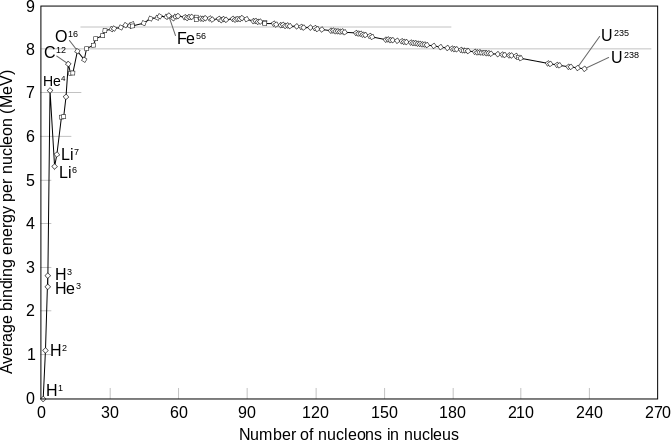
\includegraphics[width=0.9\textwidth]{../images/bindingEnergies.png}
\end{center}
\begin{parts}
	\part She combines $^3He$ to create $^{6}Li$. Overall, would this release or require energy?
		\begin{TheSolution}
			\textbf{Release Energy.} The binding energy for lithium-6 is greater than that for helium-3, meaning that it would take more energy to break apart oxygen than helium. Conversely, it would release more energy to form lithium than helium, meaning that to combine helium from lithium it would release energy.
		\end{TheSolution}
	\part She breaks apart $^{238}U$ to create $^{6}Li$. Overall, would this release or require energy?
		\begin{TheSolution}
			\textbf{Require Energy.} The binding energy for lithium-6 is less than that for uranium-238, meaning that it would take more energy to break apart uranium than lithium. Conversely, it would release more energy to form uranium than lithium, meaning that to break apart uranium to form lithium it would require energy.
		\end{TheSolution}
\end{parts}
\end{questions}


\end{document}